\chapter{交变电流 传感器}
\section{交变电流的产生及其变化规律}

1.交变电流及其产生和图象

(1)交变电流

\ding{172}定义:\_\_大小\_\_和\_\_方向\_\_都随时间做周期性变化的电流.

\ding{173}图象:如图甲、乙、丙、丁所示都属于交变电流.其中按正弦规律变化的交变电流叫\_\_正弦式\_\_交变电流,如图甲所示.

\begin{center}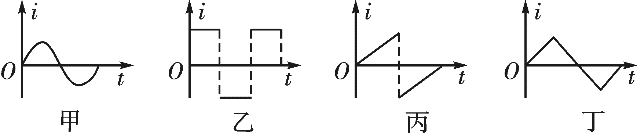
\includegraphics[width=2.89653in,height=0.60347in]{media/image436.png}\end{center}

(2)正弦交变电流的产生和图象

\ding{172}产生:在匀强磁场里,线圈绕\_\_垂直于磁场\_\_方向的轴匀速转动.

\ding{173}图象:用以描述交变电流随时间变化的规律,如果线圈从中性面位置开始计时,其图象为正弦曲线.如图甲、乙所示.

\begin{center}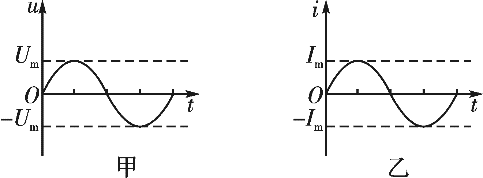
\includegraphics[width=2.19792in,height=0.81111in]{media/image437.png}\end{center}

2.正弦式交变电流的描述

(1)周期和频率

\ding{172}周期(T):交变电流完成一次周期性变化(线圈转一周)所需的时间,单位是秒(s),公式$T=\dfrac{2 \pi}{\omega}$.

\ding{173}频率(f):交变电流在1 s内完成周期性变化的次数.单位是赫兹(Hz).

\ding{174}周期和频率的关系:$T=\dfrac{1}{f}$ 或 $f=\dfrac{1}{T}$.

(2)正弦式交变电流的函数表达式(线圈在中性面位置开始计时)

\ding{172}电动势e随时间变化的规律:$e=E_{\mathrm{m}} \sin \omega t$.其中$\omega$等于线圈转动的角速度,$E_{\mathrm{m}}=n B S \omega$.

\ding{173}负载两端的电压u随时间变化的规律:$u=U_{\mathrm{m}} \sin \omega t$.

\ding{174}电流i随时间变化的规律:$i=I_{\mathrm{m}} \sin \omega t$.

(3)交变电流的瞬时值、峰值、有效值

\ding{172}瞬时值:交变电流某一时刻的值,是时间的函数.

\ding{173}峰值:交变电流(电流、电压或电动势)所能达到的最大的值,也叫最大值.

\ding{174}有效值:跟交变电流的热效应等效的恒定电流的值叫做交变电流的有效值.对正弦交流电,其有效值和峰值的关系为:$E=\dfrac{E_{\mathrm{m}}}{\sqrt{2}}, \quad U=\dfrac{U_{\mathrm{m}}}{\sqrt{2}}, I=\dfrac{I_{\mathrm{m}}}{\sqrt{2}}$.
\newpage
\subsection{正弦交变电流的产生及其变化规律}

1.正弦式交变电流的变化规律(线圈在中性面位置开始计时)

\begin{longtable}[]{@{}m{1.5cm}m{5cm}m{3cm}@{}}
\toprule
& 函数 & 图象\tabularnewline
\midrule
\endhead
磁通量 & $\Phi=\Phi_m\cos \omega t=BS\cos  \omega t$ &
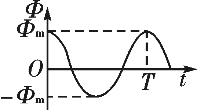
\includegraphics[width=0.89653in,height=0.5in]{media/image439.png}\tabularnewline
电动势 & $e=E_m\sin \omega t=nBS\omega\sin \omega t $&
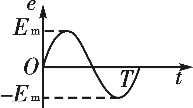
\includegraphics[width=0.87708in,height=0.49028in]{media/image440.png}\tabularnewline
电压 & $u=U_m\sin \omega t=\sin \omega t$ &
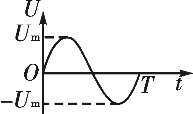
\includegraphics[width=0.87708in,height=0.51875in]{media/image441.png}\tabularnewline
电流 & $i=I_m\sin \omega t=\sin \omega t$ &
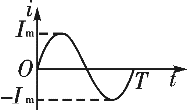
\includegraphics[width=0.84931in,height=0.5in]{media/image442.png}\tabularnewline
\bottomrule
\end{longtable}

2.两个特殊位置的特点

(1)线圈平面与中性面重合时,S$\perp$B,$\Phi$最大,$\dfrac{\Delta \Phi}{\Delta t}=0, e=0, i=0$,电流方向将发生改变.

(2)线圈平面与中性面垂直时,S$\parallel$B,$\Phi=0$,$\dfrac{\Delta \Phi}{\Delta t}$ 最大, $e$ 最大 $, i$ 最大,电流方向不改变.

(3)电流方向的改变:线圈通过中性面时,电流方向发生改变,一个周期内线圈两次通过中性面,因此电流的方向改变两次.

\begin{center}
\includegraphics[width=0.70764in,height=0.12292in]{media/image34.png}\end{center}
\begin{center}
	\textbf{解决交变电流图象问题的三点注意}
\end{center}

(1)只有当线圈从中性面位置开始计时,电流的瞬时值表达式才是正弦形式,其变化规律与线圈的形状及转动轴处于线圈平面内的位置无关.

(2)注意峰值公式$E_m=nBS\omega$中的S为有效面积.

(3)在解决有关交变电流的图象问题时,应先把交变电流的图象与线圈的转动位置对应起来,再根据特殊位置求特殊解.

{[}例1{]}如图甲为小型旋转电枢式交流发电机的原理图,其矩形线圈在磁感应强度为B的匀强磁场中,绕垂直于磁场方向的固定轴$OO^\prime$匀速转动,线圈的两端经集流环和电刷与$R=10\Omega$的电阻连接,与电阻R并联的交流电压表为理想电压表,示数是10
V.图乙是矩形线圈中磁通量$\Phi$随时间t变化的图象.则( C )

\begin{center}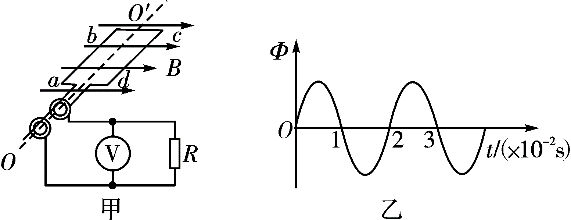
\includegraphics[width=2.59444in,height=1in]{media/image443.png}\end{center}

A.电阻R上的电功率为20 W

B.t=0.02 s时R两端的电压瞬时值为零

C.R两端的电压u随时间t变化的规律是$u=14.1\cos 100\pi t $V

D.通过R的电流i随时间t变化的规律是$i=14.1\cos 50\pi t $A

\subsection{交变电流``四值''的理解及应用}

1.交变电流的瞬时值、峰值、有效值和平均值的比较

\begin{longtable}[]{@{}m{1.2cm}m{2.5cm}m{2.5cm}m{6cm}@{}}
\toprule
物理量 & 物理含义 & 重要关系 & 适用情况及说明\tabularnewline
\midrule
\endhead
\begin{minipage}[t]{0.22\columnwidth}\raggedright
瞬时值\strut
\end{minipage} &交变电流某一时刻的值 &$e=E_{\mathrm{m}} \sin \omega t$

$i=I_{\mathrm{m}} \sin \omega t$& 
计算线圈某时刻的受力情况\tabularnewline
\begin{minipage}[t]{0.22\columnwidth}\raggedright
峰值\strut
\end{minipage} & 
最大的瞬时值&$E_{\mathrm{m}} =n B S \omega$ 

 $I_{\mathrm{m}} =\dfrac{E_{\mathrm{m}}}{R+r} $&
讨论电容器的击穿电压\tabularnewline
\begin{minipage}[t]{0.22\columnwidth}\raggedright
有效值\strut
\end{minipage} &跟交变电流的热效应等效的恒定电流的值& 

$E=\dfrac{E_{\mathrm{m}}}{\sqrt{2}}$

$U=\dfrac{U_{\mathrm{m}}}{\sqrt{2}}$

$I=\dfrac{I_{\mathrm{m}}}{\sqrt{2}}$

(只适用于正弦式交变电流)&
(1)计算与电流的热效应有关的量(如电功、电功率、电热等).(2)电器设备``铭牌''上所标的一般是指有效值.(3)保险丝的熔断电流为有效值.(4)交流电压表和电流表的读数为有效值\tabularnewline
\begin{minipage}[t]{0.22\columnwidth}\raggedright
平均值\strut
\end{minipage} & 交变电流图象中图线与时间轴所夹的面积与时间的比值& $ \bar{E} =B \bar{l} \bar{v}$

$ \bar{E} =n \dfrac{\Delta \Phi}{\Delta t} $

$ \bar{I} =\dfrac{\bar{E}}{R+r} $&
计算通过电路截面的电荷量\tabularnewline
\bottomrule
\end{longtable}

2.对交变电流有效值的理解

(1)交变电流的有效值是根据电流的热效应(电流通过电阻生热)进行定义的,所以进行有效值计算时,要紧扣电流通过电阻生热(或热功率)进行计算.

(2)注意``三同'':``相同电阻'',``相同时间''内产生``相同热量''.

(3)计算时``相同时间''一般取一个周期.

\begin{center}
\includegraphics[width=0.70764in,height=0.12292in]{media/image25.png}\end{center}
\begin{center}
	\textbf{书写交变电流瞬时值表达式的基本思路}
\end{center}


(1)求出角速度$\omega$,$\omega=\dfrac{2 \pi}{T}=2 \pi f$.

(2)确定正弦交变电流的峰值,根据已知图象读出或由公式$E_{\mathrm{m}}=n B S \omega$求出相应峰值.

(3)明确线圈的初始位置,找出对应的函数关系式.

\ding{172}线圈从中性面位置开始转动,则i-t图象为正弦函数图象,函数式为$i=I_{\mathrm{m}} \sin \omega t$.

\ding{173}线圈从垂直中性面位置开始转动,则i-t图象为余弦函数图象,函数式为$i=I_{\mathrm{m}} \cos \omega t$.
\newpage
\section{变压器的原理 电能的输送}

1.理想变压器

(1)原理:利用电磁感应的\_\_互感\_\_现象.

(2)基本关系式

\ding{172}功率关系:$P_{\text{入}}=P_{\text {出 }}$;

\ding{173}电压关系:只有一个副线圈时,$\dfrac{U_{1}}{n_{1}}=\dfrac{U_{2}}{n_{2}}$;

有多个副线圈时$\dfrac{U_{1}}{n_{1}}=\dfrac{U_{2}}{n_{2}}=\ldots$;

\ding{174}电流关系:只有一个副线圈时,$\dfrac{I_{1}}{I_{2}}=\dfrac{n_{2}}{n_{1}}$;

由$P_{\text{入}}=P_{\text {出 }}$及$P=UI$推出有多个副线圈时,$U_{1} I_{1}=U_{2} I_{2}+U_{3} I_{3}+\ldots+U_{n} I_{n}$.

(3)常用的变压器

\ding{172}自耦变压器------调压变压器;

\ding{173}互感器
电压互感器:用来把高电压变成低电压.

电流互感器:用来把大电流变成小电流.


2.远距离输电

(1)输电过程(如图所示)

\begin{center}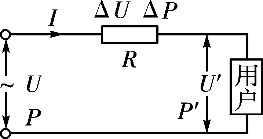
\includegraphics[width=1.19792in,height=0.63194in]{media/image450.png}\end{center}

(2)输电导线上的能量损失:主要是由输电线的电阻发热产生的,表达式为$Q=I^2Rt$.

(3)电压损失

\ding{172}$\Delta U=U-U^\prime$;\ding{173}$\Delta U=IR$.

(4)功率损失

\ding{172}$\Delta P=P-P^\prime$;\ding{173}$\Delta P=I^2R=(\dfrac{P}{U})^2R$.

(5)输送电流

\ding{172}$I=\dfrac{P}{U}$;\ding{173}$I=\dfrac{U-U^\prime}{R}$.
\newpage
\subsection{理想变压器的特点与制约关系}

1.理想变压器的特点

(1)没有能量损失(铜损,铁损).

(2)没有磁通量损失(磁通量全部集中在铁芯中).

2.制约关系

(1)电压制约关系:副线圈电压$U_2$由原线圈电压$U_1$和匝数比决定.

(2)电流制约关系:原线圈电流$I_1$由副线圈电流$I_2$和匝数比决定.

(3)功率制约关系:原线圈的输入功率$P_1$由副线圈的输出功率$P_2$决定.

\begin{center}
\includegraphics[width=0.70764in,height=0.12292in]{media/image34.png}\end{center}
\begin{center}
	\textbf{关于理想变压器的四点说明}
\end{center}

(1)变压器不能改变恒定的直流电压.

(2)变压器只能改变交变电流的电压和电流,不能改变交变电流的频率.

(3)理想变压器本身不消耗能量.

(4)当原线圈中串联电阻(或灯泡)时,$U_1$为加在原线圈两端的电压,并不是电源的电压.

{[}例1{]}(2017·北京卷)如图所示,理想变压器的原线圈接在$u=220 \sqrt{2} \sin 100 \pi t \mathrm{V}$的交流电源
上,副线圈接有R =55
$\Omega$的负载电阻,原、副线圈匝数之比为2:1,电流表、电压表均为理想电表.下列说法正确的是( B )
\begin{center}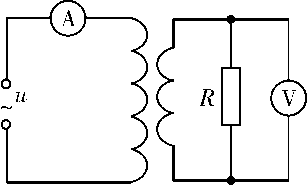
\includegraphics[width=1.39653in,height=0.83958in]{media/image451.png}\end{center}

A.原线圈的输入功率为220 W

B.电流表的读数为1 A

C.电压表的读数为110 V

D.副线圈输出交流电的周期为50 s
\begin{solution}
	B
	
	由交流电压的表达式可知,原线圈两端所加的电压最大值为$220 \sqrt{2} \mathrm{v}$,故有效值为$U_{1}=220 \mathrm{V}$,由$\dfrac{U_{1}}{U_{2}}=\dfrac{n_{1}}{n_{2}}$,故副线圈电压的有效值为$U_2=110V$,故输出功率$P_{2}=\dfrac{U_{2}^{2}}{R}=220 \mathrm{W}$,再由输入功率等于输出功率知,$P_1=P_2=220W$,选项A错误;根据欧姆定律知,$I_{2}=\dfrac{U_{2}}{R}=2 \mathrm{A}, \dfrac{I_{1}}{I_{2}}=\dfrac{n_{2}}{n_{1}}$,得$I_1=1 A$,故电流表读数为1
A,所以选项B正确;电压表的读数为有效值,即$U_2=110
V$,选项C错误;由交流电压的表达式可知,$\omega=100 \pi(\mathrm{rad} / \mathrm{s}), \quad$ 又 $T=\dfrac{2 \pi}{\omega}$,解得T=0.02
s,所以选项D项错误.
\end{solution}
\newpage
\subsection{理想变压器的动态分析}

1.匝数比不变的情况(如图所示)

\begin{center}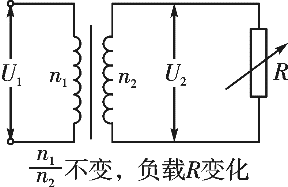
\includegraphics[width=1.31111in,height=0.84931in]{media/image452.png}\end{center}

(1)$U_1$不变,根据$\dfrac{U_{1}}{U_{2}}=\dfrac{n_{1}}{n_{2}}$,输入电压$U_1$决定输出电压$U_2$,不论负载电阻R如何变化,$U_2$也不变.

(2)当负载电阻发生变化时,$I_2$变化,输出电流$I_2$决定输入电流$I_1$,故$I_1$发生变化.

(3)$I_2$变化引起$P_2$变化,$P_1$=$P_2$,故$P_1$发生变化.

\begin{center}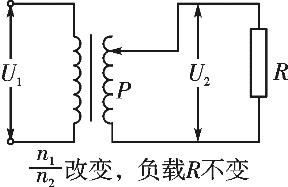
\includegraphics[width=1.31111in,height=0.84931in]{media/image453.png}\end{center}

2.负载电阻不变的情况(如图所示)

(1)$U_1$不变,$\dfrac{n_{1}}{n_{2}}$发生变化,故$U_2$变化.

(2)R不变,$U_2$改变,故$I_2$发生变化.

(3)根据$P_{2}=\dfrac{U_{2}}{R}$,$P_2$发生变化,再根据$P_1=P_2$,故$P_1$变化,$P_1=U_1I_1$,$U_1$不变,故$I_1$发生变化.

\begin{center}
\includegraphics[width=0.70764in,height=0.12292in]{media/image25.png}\end{center}
\begin{center}
	\textbf{含有变压器的动态电路分析方法}
\end{center}

(1)确定原线圈电压$U_1$$\rightarrow$原线圈电压$U_1$为定值

(2)确定副线圈电压$U_2$$\rightarrow$由$U_{2}=\dfrac{n_{2}}{n_{1}} U_{1}$知,若$n_1$、$n_2$为定值,$U_2$也为定值

(3)确定副线圈电流$I_2$$\rightarrow$由 $I_{2}=\dfrac{U_{2}}{R}$ 知 $, \quad R$ 增大时 $, I_{2}$ 减小

(4)确定输出功率$P_2$$\rightarrow$由 $P_{2}=I_{2} U_{2}$ 知口 $, I_{2}$ 减小时 $, P_{2}$ 喊小

(5)确定输入功率$P_1$$\rightarrow$由 $P_{1}=P_{2}$ 知, $P_{2}$ 减小 $, P_{1}$ 也减小

(6)确定原线圈电流$I_1$$\rightarrow$由 $I_{1}=\dfrac{P_{1}}{U_{1}}$ 知 $, \quad P_{1}$ 哲小小时 $, \quad I_{1}$ 协咸小


\newpage
\subsection{三种特殊的变压器模型}

1.自耦变压器

自耦变压器(又称调压器),它只有一个线圈,其中的一部分作为另一个线圈,当交流电源接不同的端点时,它可以升压也可以降压,变压器的基本关系对自耦变压器均适用,如图所示.

\begin{center}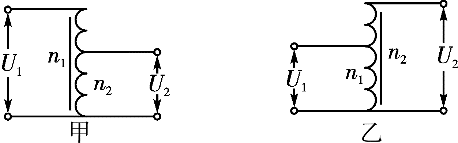
\includegraphics[width=2.08472in,height=0.65069in]{media/image455.png}\end{center}

2.互感器

分为电压互感器和电流互感器,比较如下:

\begin{longtable}[]{@{}m{2.2cm}m{4cm}m{4cm}@{}}
\toprule
& 电压互感器 & 电流互感器\tabularnewline
\midrule
\endhead
原理图 &
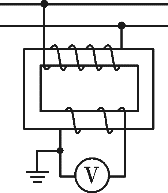
\includegraphics[width=0.76389in,height=0.87708in]{media/image458.png} &
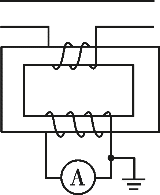
\includegraphics[width=0.72639in,height=0.88681in]{media/image459.png}\tabularnewline
原线圈的连接 & 并联在高压电路中 & 串联在交流电路中\tabularnewline
副线圈的连接 & 连接电压表 & 连接电流表\tabularnewline
互感器的作用 & 将高电压变为低电压 & 将大电流变成小电流\tabularnewline
利用的公式 & $\dfrac{U_{1}}{U_{2}}=\dfrac{n_{1}}{n_{2}}$ & $I_{1} n_{1}=I_{2} n_{2}$\tabularnewline
\bottomrule
\end{longtable}




3.$\Box\Box$ 字形铁芯变压器
\begin{center}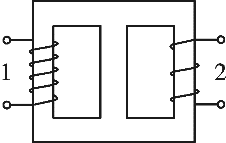
\includegraphics[width=1.02847in,height=0.65069in]{media/image461.png}\end{center}

如图所示,将两个线圈绕在图示变压器的铁芯的左、右两个臂上,当通以交流电时,每个线圈产生的磁通量都有一半通过另一个线圈,另一半通过中间臂.线圈1为原线圈时,穿过线圈1的每一匝线圈的磁通量只有一半通过线圈2的每一匝线圈,所以穿过线圈2的每一匝线圈的磁通量的变化率也只有穿过线圈1的每一匝线圈的磁通量的变化率的一半.由$U_1=E_1=n_{1} \dfrac{2 \Delta \Phi}{\Delta t}, \quad U_{2}=E_{2}=n_{2} \dfrac{\Delta \Phi}{\Delta t}$ 得 $\dfrac{U_{1}}{U_{2}}=\dfrac{2 n_{1}}{n_{2}}$.


\newpage
\subsection{远距离输电}

1.理清三个回路

\begin{center}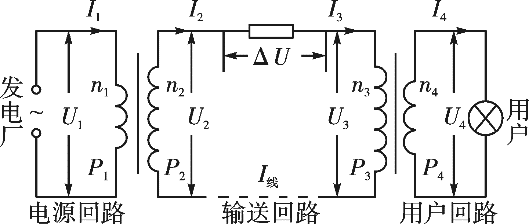
\includegraphics[width=2.40556in,height=1.01875in]{media/image463.png}\end{center}

远距离输电电网间的基本结构,如图所示.输电过程的电路被划分为三个独立的回路,即电源回路、输送回路和用户回路.在每个回路中,变压器的原线圈是回路的用电器,而相应的副线圈是下一个回路的电源,每个回路均可应用闭合电路欧姆定律、串并联电路的规律,而变压器的电压、电流、功率关系则是联系不同回路的桥梁.

2.抓任两个联系

(1)理想的升压变压器联系了电源回路和输送回路,由理想变压器原理可得:线圈1(匝数为$n_1$)和线圈2(匝数为$n_2$)中各个量间的关系是$\dfrac{U_{1}}{U_{2}}=\dfrac{n_{1}}{n_{2}}, I_{1} n_{1}=I_{2} n_{2}, P_{1}=P_{2}$.

(2)理想的降压变压器联系了输送回路和用户回路,由理想变压器原理可得:线圈3(匝数为$n_3$)和线圈4(匝数为$n_4$)中各个量间的关系是$\dfrac{U_{3}}{U_{4}}=\dfrac{n_{3}}{n_{4}}, \quad I_{3} n_{3}=I_{4} n_{4}, \quad P_{3}=P_{4}$.

3.掌握一个能量守恒定律

发电机把机械能转化为电能,并通过导线将能量输送给线圈1,线圈1上的能量就是远程输电的总能量,在输送过程中,先被输送回路上的导线电阻损耗一小部分,剩余的绝大部分通过降压变压器和用户回路被用户使用消耗,所以其能量关系为$P_{1}=P_{\text {线损 }}+P_{\text {用户 }}$ .

\begin{center}
\includegraphics[width=0.70764in,height=0.12292in]{media/image13.png}\end{center}
\begin{center}
	\textbf{解决远距离输电问题应注意下列几点}
\end{center}

(1)画出输电电路图.

(2)注意升压变压器副线圈中的电流与降压变压器原线圈中的电流相等.

(3)输电线长度等于距离的2倍.

(4)计算线路功率损失一般用$P_{\text {损 }}=I_{\text {线 }}^2R_{\text {线 }}$.
